\chapter{Implementierung}
%Was genau soll implementiert werden
Im Kapitel \sref{sec:t_grund} wurden die Grundlagen zu den \gls{ml}-Algorithmen erklärt.  
In diesem Kapitel werden alle erforderlichen Komponenten implementiert, um ML-Modelle zur Vorhersage von Waitinglist-Entscheidungen zu trainieren.
\section{Datenaggregation via Databricks}
%Warum müssen die Daten aggregiet werden?
Die \gls{ml}-Modelle sollen überwacht trainiert werden.  
Im Rahmen dieser Arbeit erfolgt das Training der Modelle auf der Basis vergangener Entscheidungen.

%\todo{IW: überwachtes training}
%heißt auf Deutsch "überwacht".
%Auch supervised könnte man noch als technischen Begriff gelten lassen, aber dann müssen Sie auch weiter oben deutlich erklären und gegen unsupervised abgrenzen.

%Supervised: Ich ging davon aus, dass das nicht hier extra erwähnt werden muss.
%Im übrigen haben Sie supervised in den Grundlagen gar nicht erklärt, sodass das hier auch nichts mehr bringt. Wenn Sie also den Unterschied von überwacht zu unüberwacht thematisieren wollen (wogegen ich nichts habe), dann vorher in den theoretischen Grundlagen mit der Erwähnung, dass es sich hier offenbar um ein Problem handelt, welches ein überwachtes Lernen voraussetzt. Das ist auch nicht verwunderlich, denn Sie wollen ja nicht Daten sortieren, sondern auf gewisse Eingaben Ergebnisse vorhersagen.

Hierfür muss zunächst ein Datensatz erstellt werden. 
Dabei sind nicht nur die Entscheidungen selbst, sondern auch die relevanten Entscheidungsfaktoren erforderlich.
Für die Aggregation und Speicherung dieser historischen Daten wurden \textbf{\nameref{sec:databricks}-SQL-Notebooks} verwendet.


%\subsection{Entscheidungsfaktoren für die Waitinglist}
%Vielleicht die Entscheidungfaktoren in Gruppeneinteilen?
%Ergklären aus welchen Tabellen man welche faktoen bekommen?
%?? Wie hängen die Daten zusammen?
%-> Viele Faktoren sind nicht an der logging tabelle

%Ob eine Buchung von der Waitinglist angenommen oder Abgelehnt wird, kommt auf viele Faktoren an. 
%Als Ausgangspunkt werden die Daten, welche auf dem A1050 enthalten sind, verwendet. 
%Hinzugefügt wurden noch weiter Eigenschaften, welche auf die Entscheidung, Einfluss haben könnten. 
%\todo{IW: Tabelle weiter nach oben}


\subsection{Probleme}
Auf Basis der vorgestellten Eigenschaften (\cref{tab:waitinglistattr}), sollen die historischen Daten aus dem Data Lake geladen werden. Es wurde als Basistabelle die Loggingtabelle \gls{ts2390} gewählt, denn diese enthält alle \hyperref[ref:announcement]{Annoucment}-Ergebnisse. Also auch die Information, wenn eine Buchung von der Waitinglist angenommen oder abgelehnt wurde. 

Bei jeder Entscheidung werden schon direkt viele Eigenschaften mit in die \gls{ts2390} geschrieben, jedoch nicht alle benötigten.
Daher müssen die fehlenden Informationen aus weiteren Tabellen ergänzt werden, um einen vollständigen Datensatz zu erhalten.

%\todo{IW: JOIN mengentheorie}
%Erklären Sie hier kurz, was JOIN mengentheoretisch macht.


\subsubsection{Tabellenbenennung}

Um aus den verschiedenen Tabellen eine Abfrage zu erstellen, ist es notwendig, die Tabellen eindeutig zu identifizieren. 
Dabei treten jedoch die ersten Herausforderungen auf: Bei \gls{hl} besitzen die Tabellen ausschließlich technische Namen. 
In diesem Fall hat jede der über $1400$ Tabellen einen Namen, der aus zwei Buchstaben gefolgt von einer Nummer besteht. 
Beispiele hierfür sind \gls{ts2390} oder \gls{ts0340}. 
Zusätzlich zu diesen Namen gibt es auch fachliche Bezeichnungen, jedoch sind diese in der Datenbank selbst nicht sichtbar.
Durch mangelnde Dokumentation ist es schwierig, die richtigen Tabellen zu einem fachlichen Thema zu finden.

Um dieses Problem zu umgehen, werden drei Ansätze verfolgt. 
Zum einen kann in der Codebasis von \gls{fis}3 recherchiert werden. 
Alternativ ist es möglich, im externen Werkzeug \enquote{Collibra} nach einer fachlichen Bezeichnung zu suchen.

%\todo{IW: Collibra erwähnen}
%Wenn Sie Collibra hier namentlich erwähnen, müssen Sie oben bei der fachlichen Beschreibung erwähnen, was in Collibra zu welchem Zweck abgelegt ist.

Schließlich besteht auch die Möglichkeit, sich direkt an erfahrene Mitarbeiter zu wenden, die aufgrund ihrer langjährigen Tätigkeit viele der Tabellen in ihrem Bereich auswendig kennen.
Letzteres wurde größtenteils verwendet, aber in Kombination mit den anderen Methoden.

\subsubsection{Historische Daten (Bronze-Zone)}
%Warum müssen wir joinen?
In der \gls{ts2390}-Tabelle befinden sich die vergangenen Entscheidungen aller \hyperref[ref:announcement]{Annoucments}. Dabei fehlen aber noch viele Informationen, da die \gls{ts2390} eine Logging-Tabelle ist.  
Allgemein dienen solche Tabellen dazu, Änderungen, Ereignisse oder Aktivitäten in einem System zu protokollieren, um Nachverfolgbarkeit und Fehleranalysen zu ermöglichen.  
In diesem Fall speichert die \gls{ts2390} spezifisch die Entscheidungen der Waitinglist-Bearbeitung, enthält jedoch nicht alle für die weitere Verarbeitung relevanten Informationen.

Dies kann gut an dem \hyperref[ref:attr_ssy]{Schiffsystem-Attribut} veranschaulicht werden. 
Das Attribut wird nicht direkt in der \gls{ts2390}-Tabelle als Spalte abgelegt, sondern nur die \gls{dpvno}. 
Über die \gls{dpvno} kann das Schiff in der \gls{tt0004}-Tabelle gefunden werden. 
An dem Schiff hängt dann erst das Schiffssystem-Attribut.
Es muss also die \gls{ts2390} mit der \gls{tt0004} verbunden werden. 

%Wie würde man in Silber joinen
Da die \gls{dpvno}-Spalte einzigartig ist, kann maximal die gleiche Spaltenanzahl der \gls{ts2390} erreicht werden. Es können alle, über Schlüsselattribute verknüpften Tabellen gejoint werden, ohne dass sich die Anzahl der Ergebniszeilen vergrößert. Das bedeutet, dass eine 1:1-Beziehung besteht.

%Warum braucht man die Bronze Zone
Bei einer Logging-Tabelle ist zu beachten, dass die Logging-Daten sich nicht auf den aktuellen Stand der Datenbank beziehen, sondern auf den Zeitpunkt der Zeilenerstellung. Als Beispiel: 

In der Logging-Tabelle \gls{ts2390} ist eine Waitinglist-Entscheidung gespeichert. 
Um das \hyperref[ref:attr_kunde]{Kunden-Attribut} zur Entscheidung auszulesen, muss die zugehörige Buchung verknüpft werden.  
Da ein Buchungseintrag im Durchschnitt $140$ Mal verändert wird, kann es zu Abweichungen kommen, wenn die aktuelle Buchung statt der zum Entscheidungszeitpunkt gültigen Version selektiert wird.
Daher muss auf die \hyperref[tab:zonenbsp]{Bronze-Zone} zurückgegriffen werden, denn dort sind alle Änderungen vorhanden.

%Warum kann man nicht einfach das nicht in Bronze wie in Silver machen?
Die Komplexität besteht darin, dass nicht mehr über das Schlüsselattribut eine 1:1-, sondern eine 1:n-Beziehung besteht. 
In diesem Fall bedeutet das, dass ein Logging-Eintrag aus der \gls{ts2390} mit mehreren Versionen einer Buchung (\gls{ts0340}) verbunden wird.

Es gibt jedoch zu jedem Logging-Eintrag (\textit{Waitinglist-Entscheidung}) genau eine passende Zeile (\textit{Version der Buchung}): die neueste Zeile, die zeitlich vor der Entscheidung liegt.

\begin{table}[H]
    \centering
    \begin{tabular}{cc|ccc}
        \hline\hline
        \multicolumn{2}{c|}{\thead{\gls{ts2390}}}&  \multicolumn{3}{c}{\gls{ts0340}}\\
        \hline
        \thead{Datum}&  Buchungsnummer &  Nummer& Kundennummer &Änderungsdatum\\
        \hline
        01.06.2024&   \textbf{\textcolor{hlblue}{1}}&  \textbf{\textcolor{hlblue}{1}}& 1 &25.05.2024\\
        &&  \cellcolor{hlorange}\textbf{\textcolor{hlblue}{1}}&  \cellcolor{hlorange}2&\cellcolor{hlorange}26.05.2024\\
        && \textbf{\textcolor{hlblue}{1}}& 3&02.01.2024\\
        \multicolumn{2}{c|}{...}& \multicolumn{3}{c}{...}\\
        \hline\hline
    \end{tabular}
    \caption{Beispiel: Logging-Tabelle (\gls{ts2390}) zu Buchungstabelle (\gls{ts0340})}
    \label{tab:prob_hist_eg}
\end{table} 

%Wie wurden die joins aus Silber in Bronze umgesetzt\\
Um genau diese Buchung zu finden, muss komplexer verfahren werden. Es wird zusätzlich zu de(n/m) Primärschlüssel(n) noch der Änderungszeitpunkt der Zeile benötigt, um eine Zeile eindeutig zu identifizieren. 
Die Query wird so aufgeteilt, dass zunächst die benötigten Primärschlüssel mit den Änderungszeitpunkten gefunden werden und danach diese mit der Tabelle gejoint werden. 
Um diese zu sammeln, wird die \gls{ts2390} mit jeder Tabelle zusammengefügt (\lstinline[language=SQL]|JOIN|).
Es wird hierbei in der \lstinline[language=SQL]|JOIN ON| Bedingung festgelegt, dass der Änderungszeitpunkt jünger/kleiner als der Entscheidungszeitpunkt ist. 
Dabei werden nur die Primärschlüssel und zusätzlich über eine Aggregationsfunktion das Maximum des Änderungsdatums selektiert. 
Anschließend werden die Daten nach Primärschlüsseln gruppiert, sodass man jeden Primärschlüssel mit dem neuesten Zeitpunkt erhält, der vor der Entscheidung liegt.
\begin{figure}[H]
    \centering
    \begin{lstlisting}[language=SQL]
      SELECT 
        shipment.NUMBER, -- Primaerschluessel vom Shipment
        max(dpvoyage.header__event_timestamp_string) as voyage_timestamp
      [...]
      FROM "TS2390" announcement_result
      JOIN "TS0340" shipment on (
        shipment.NUMBER = announcement_result.SHIPMENT_NUMBER 
        and shipment.header__event_timestamp_string <= announcement_result.ACTION_TIMESTAMP
      )
      [...]
      GROUP BY shipment.NUMBER [...]
    \end{lstlisting}
    \caption{SQL-Statement: Selektion der Primärschlüssel mit dazugehörigem Zeitstempel}
    \label{fig:hidden_layer_struct}
\end{figure}



\subsubsection{Join mit großen Tabellen}
In der Bronze-Zone liegt eine vielfach höhere Anzahl an Zeilen im Vergleich zur produktiven Datenbank vor (siehe \ref{tab:tab_sizes}).

Da bei einem \lstinline[language=SQL]|JOIN| vorgefiltert werden soll, wurden erstmals aus allen verwendeten Tabellen gefilterte Vortabellen erstellt. 
Herausgefiltert wurden hierbei alle Zeilen, die definitiv nicht für die Weiterbearbeitung nötig waren. 

Zum Beispiel wurden alle Announcement-Ergebnisse, die einen Statuswechsel von der Waitinglist zu angenommen/abgelehnt beinhalten, in eine neue Tabelle namens \enquote{relevant\_annoucment\_results} geschrieben. 
Es wurden also alle nicht relevanten Announcement-Ergebnisse herausgefiltert. 
Danach wurden alle Buchungen, die in der \enquote{relevant\_annoucment\_results} referenziert wurden, als \enquote{relevant\_shipments} Tabelle gespeichert. 
Dadurch wurde die durchschnittliche Tabellenzeilenanzahl um \hyperref[tab:tab_sizes_diff]{78,75\%} reduziert. 
Dies wurde mit allen nötigen Tabellen fortgeführt.

Als weitere Optimierung wurde mit dem \lstinline[language=SQL]|WITH| Operator auf temporäre Zwischentabellen zurückgegriffen \cite{Horvat2008}. Wenn alle Tabellen in einem Statement für die Suche nach Primärschlüsseln und Änderungszeitpunkten zusammengefügt werden, entsteht zunächst eine große Anzahl an Zeilenkombinationen. Erst durch die anschließende Gruppierung wird diese reduziert.
Dabei muss die Gruppierung alle zuvor entstandenen Kombinationen durchlaufen.

Beispiel:
Es wird berechnet, wie viele Zeilen maximal bei der \lstinline[language=SQL]|JOIN|-Operation entstehen, wenn alle zuvor gefilterten Tabellen miteinander gejoint werden:

\[
\begin{array}{r}
   3.588.837 \\
   1.063.926.886 \\
   495.985.080 \\
   159.816.410 \\
\times 387.841.791 \\
    \hline
   1\text{,}1738 \times 10^{41}
\end{array}
\]
Die Ergebnismenge muss dann gruppiert und somit wieder auf die 3.588.837 Announcement-Ergebnis-Zeilen reduziert werden. Aufgrund der großen Anzahl an Zeilen kann die Gruppierung nicht direkt durchgeführt werden.


Wenn man aber in Zwischentabellen jeweils nach einem \lstinline[language=SQL]|JOIN| immer direkt gruppiert, kann man die zu gruppierenden Zeilen erheblich reduzieren:

\resizebox{\textwidth}{!}{
    $\begin{array}{cccc}
        \begin{array}{r}
            3.588.837 \\
            \times 1.063.926.886 \\
            \hline
            \textcolor{hlorange}{3.818.260.173.771.580}
        \end{array}
        &
        \begin{array}{r}
            3.588.837 \\
            \times 495.985.080 \\
            \hline
             1.780.009.606.551.960 
        \end{array}
        &
        \begin{array}{r}
            3.588.837 \\
            \times 159.816.410 \\
            \hline
            573.555.045.415.170 
        \end{array}
        &
        \begin{array}{r}
            3.588.837 \\
            \times 387.841.791 \\
            \hline
            1.391.900.969.687.070
        \end{array}
    \end{array}$
}

Hierbei zeigt sich, dass maximal $3\text{,}8182 \times 10^{15}$ Zeilen gruppiert werden, was nur noch $(3\text{,}25 \times 10^{-24})\%$ des vorherigen Ansatzes sind.
%\todo{IW: Datenbanktheorie muss in die Grundlagen}
%Sie setzen hier Datenbankwissen voraus, obwohl offenbar eine spezielle Datenhaltung bei HL eines Ihrer Hauptprobleme zu sein scheint.
%Offenbar ist Datenbankwissen für Ihre Lösung erforderlich. Daher sollten Sie das in den Grundlagen auch beschreiben und darauf aufbauend den Istzustand in diesem Kapitel, auf den Sie dann mit den genannten Maßnahmen reagieren müssen.

\subsection{Query}
Unter Berücksichtigung der genannten Komplexitäten ist das Ergebnis eine Query, die über $12$ temporäre Zwischentabellen via \lstinline[language=SQL]|WITH|, die historischen Primärschlüssel mit Zeitstempel sucht und in der finalen Selektion diese Schlüssel verwendet, um die relevanten Daten zu joinen. 
Die Query ist dabei über $720$ Zeilen lang (siehe \ref{sec:extdrive}).
Es wird daraus eine Tabelle namens \enquote{waitlisting\_data} erstellt.
Für die Ausführung wird aufgrund der Optimierungen nur noch eine Laufzeit von $20$ Minuten benötigt, wobei $3.588.646$\label{ref:dataset} historische Waitinglist-Entscheidungen resultieren. 
Diese bestehen aus $2.469.976$ Annahmen und $1.118.670$ Ablehnungen. 
Das bedeutet, dass mehr als doppelt so viele Annahmen wie Ablehnungen gibt.
Der Datensatz ist also \textbf{nicht ausgeglichen}.
Die Entscheidungen umfassen $49$ Spalten: die Ergebnis-Spalte, \hyperref[tab:waitinglistattr]{Entscheidungsfaktoren} in $35$ Spalten und dazu $13$ Spalten für Debugging-Zwecke. 
Dieser Datensatz wird für die Experimente genutzt.

%%%%%%%%%%%%%%%%%%%%%%%%%%%%%%%%%%%%%%%%%%%%%%%%%%%%%%%%%%%%%%%
%#############################################################%
%%%%%%%%%%%%%%%%%%%%%%%%%%%%%%%%%%%%%%%%%%%%%%%%%%%%%%%%%%%%%%%
\section{Machine Learning}
%Historie -> Wie hat es begonnen?
%-> Erst Neuronale Netze, Dann Random Forest als Alternative -> Vielleicht weil frage ob NN notwendig sind... 

%Der Ablauf semtptlicher Experimente hat die gleiche Struktur:
%Laden der Daten
%Feature Engeneering
%Daten Vorbereitung für Training
% -> Aufteilen der Daten in Training und testdaten
%Modellabhänige Sachen, wie Modell Struktur
%Modell Trainieren
Sämtliche Experimente wurden in \nameref{sec:databricks}-Python-Notebooks umgesetzt, deren Aufbau grundlegend gleich ist. 

\begin{enumerate}[noitemsep]
    \item Laden des \hyperref[ref:dataset]{Datensatzes}
    \item Durchführung des Feature Engineerings (siehe \ref{sec:feature_engeneering_impl})
    \item Aufteilung der Daten in Trainings- und Testdaten
    \item Modellspezifische Definitionen
    \item Modelltraining
\end{enumerate}

Für das Laden der Daten wird \enquote{PySpark} verwendet, ein Framework in Databricks, das zur verteilten Verarbeitung und Analyse großer Datenmengen dient. Mithilfe von \enquote{PySpark} werden die Tabellen in einen \href{https://spark.apache.org/docs/latest/api/python/reference/pyspark.sql/api/pyspark.sql.DataFrame.html}{DataFrame} geladen, der anschließend für das Feature Engineering verwendet wird.


\subsection{Feature Engineering}
\label{sec:feature_engeneering_impl}

%\todo{IW: Feature Engeneering.. Features}
%Es ist ok, wenn Sie auch auf Implementierungsebene darstellen, wo Sie welche Daten herbekommen.
%Was ich aber oben und auch zum Verständnis hier vermisse:
%Welche Merkmale (Features) von Auftragsbestellungen bzw. des Navigationsumfelds bedingen welchen Status auf der Waitinglist (wobei ich ja noch nicht verstanden habe, was dort überhaupt eingetragen wird)?

Beim Feature Engineering (\cref{sec:feature_engeneering}) werden die Rohdaten transformiert, um sie möglichst informativ und effizient für das Modell zu gestalten. Dieser Prozess umfasst mehrere Schritte:

\begin{enumerate}
    \item \textbf{Datenvorverarbeitung:}  
    In dieser Arbeit wurde die Datenvorverarbeitung bereits während der Erstellung des Datensatzes durchgeführt, sodass dieser Schritt hier nicht erneut erforderlich war.

    \item \textbf{Feature-Erstellung:}  
    Bei der Feature-Erstellung werden aus bestehenden Daten neue Merkmale (Features) abgeleitet, die die Modelle besser unterstützen können. 
    Für den Waitinglist-Datensatz wurden die Spalten der \enquote{Special Products} und der \enquote{Container-Typen} in neue Features umgesetzt. Die \enquote{Special-Products} waren im Ursprung eine Liste von Produkt-Codes. Beispielsweise: \enquote{INCH} und \enquote{WQUO}. Ungeachtet genau was diese \enquote{Special-Product-Codes} sind, stehen sie separat für ein eigenes Produkt. 
    Damit dies von dem folgenden Modell unterschieden werden kann, wird die eine Spalte mit der Liste an Produkten in mehrere Spalten aufgespalten. 
    Jede dieser neuen Spalten repräsentiert ein mögliches Produkt. 
    Für jedes Produkt, das in einer Zeile enthalten ist, wird der Wert auf $1$ gesetzt, während für nicht vorhandene Produkte eine $0$ eingetragen wird.

    
    \begin{table}[H]
        \centering
        \begin{tabular}{cc|ccc}
            \hline\hline
             \multicolumn{2}{c|}{Ursprungsspalten}& \multicolumn{3}{c}{Neue Spalten}\\
             ID&  Special Products&  Hat\_INCH&  Hat\_WQUO& Hat\_BIO50\\
             \hline
             1& INCH, WQUO& 1& 1&0\\
             2& WQUO, BIO50& 0& 1&1\\
             3& & 0& 0& 0\\
            \hline\hline
        \end{tabular}
        \caption{Beispiel: Feature-Erstellung der \enquote{Special Products} Spalte}
        \label{tab:bsp_special_products}
    \end{table}

    Dieses Verfahren ähnelt sehr der \enquote{One-Hot-Kodierung}. Es wurde für die \enquote{Special Products} Spalte $67$ Features erstellt.

    Bei der \enquote{Container-Typen} Spalte wurde ein ähnliches Verfahren genutzt. 
    Es stehen in einer Spalte alle Containertypen, die in der Buchung vorhanden sind. 
    Dabei kann im Gegensatz zu den \enquote{Special Products} ein Containertyp mehrmals vorkommen. Beispielsweise kann zweimal der Containertyp \enquote{42GP} in einer Buchung vorhanden sein, weil 2 Container davon in der Buchung vorhanden sind. 
    Für diesen Fall wurde das vorherige Verfahren so abgeändert, dass wieder für jeden möglichen Typen eine neue Spalte erstellt wird, aber es nicht mehr nur eine $1$ oder $0$ in den Zellen stehen kann, sondern die Anzahl des Typen.

    \begin{table}[H]
        \centering
        \begin{tabular}{cc|ccc}
            \hline\hline
             \multicolumn{2}{c|}{Ursprungsspalten}& \multicolumn{3}{c}{Neue Spalten}\\
             ID&  Container Typen&  Hat\_42GP&  Hat\_45GP& Hat\_22GP\\
             \hline
             1& 42GP, 42GP, 22GP& 2& 0&1 \\
             2& 22GP, 42GP& 1& 0&1 \\
             3& & 0& 0& 0 \\
            \hline\hline
        \end{tabular}
        \caption{Beispiel: Feature-Erstellung der \enquote{Containertypen}-Spalte}
        \label{tab:bsp_cont_type}
    \end{table}

    Durch dieses Verfahren wurden für die \enquote{Container-Typen} Spalte $85$ Features erstellt.

    Für \enquote{Special Products} und \enquote{Container-Typen} mussten somit als Erstes alle möglichen Kategorien gesammelt werden und anschließend wurde pro Kategorie eine Spalte erzeugt. Diese neuen Spalten sind damit neue Features. Es wurde hierbei insgesamt $152$ neue Features erstellt und eine Feature-Anzahl von $181$ erreicht.

    \item \textbf{Feature-Auswahl:}  
    Für die Auswahl der Features, wurde eine Korrelationsanalyse durchgeführt, um die Feature-Anzahl zu senken. 
    \enquote{PySpark} bietet hierfür die Methode \href{https://spark.apache.org/docs/latest/api/python/reference/pyspark.sql/api/pyspark.sql.DataFrame.corr.html}{\enquote{corr}}, mit der die Korrelation zwischen zwei Spalten berechnet werden kann.
    Es wurde für eine komplette Korrelationsanalyse jede Spalte mit jeder anderen Spalte mittels der \href{https://spark.apache.org/docs/latest/api/python/reference/pyspark.sql/api/pyspark.sql.DataFrame.corr.html}{\enquote{corr}-Methode} verglichen und der Korrelationswert ermittelt.  

    \begin{figure}[H]
        \centering
        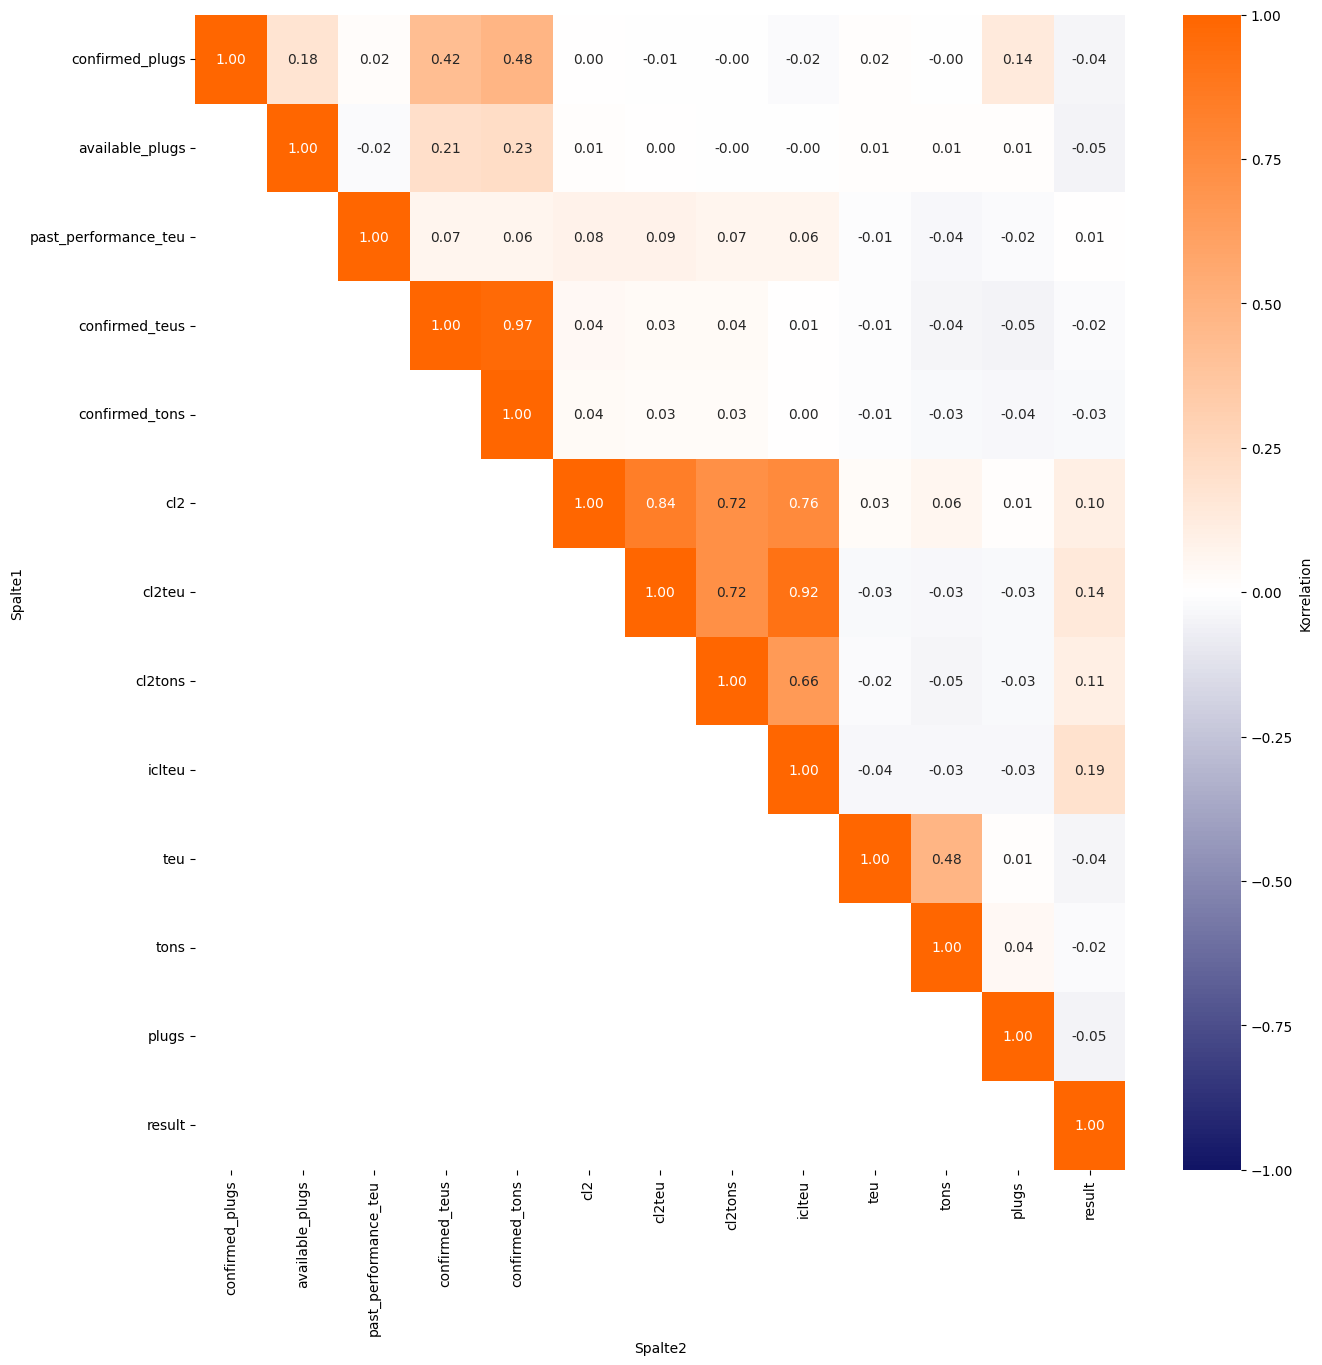
\includegraphics[width=0.85\linewidth]{Thesis//bilder/corr-analyse.png}
        \caption{Korrelationsanalyse der $29$ numerischen Features}
        \label{fig:corr_analyse}
    \end{figure}

    Bei der Korrelationsanalyse fallen die Features \enquote{cl2} und \enquote{confirmed\_teu} auf. 
    \enquote{cl2} hat mit \enquote{cl2teu}, \enquote{cl2tons} und \enquote{iclteu} eine Korrelation von jeweils über $0\text{,}7$, was zeigt, dass die Information redundant in den verschiedenen Features schon vorhanden ist.
    \enquote{confirmed\_teu} hat mit \enquote{confirmed\_tons} eine stark positive Korrelation von nahezu $0\text{,}97$.
    Daher wurden \enquote{cl2} und \enquote{confirmed\_teu} entfernt. 
    
    Features wie \enquote{cl2\_teu} oder \enquote{cl2\_tons} werden beibehalten, weil diese fachlich relevant sind.
    Bei der Entscheidung der Mitarbeiter werden beide Werte benötigt, da auf einem Schiff entweder der verfügbare Platz oder das Gewicht der limitierende Faktor sein können.
    Wenn auf einem Schiff noch ausreichend Platz vorhanden ist, aber die Gewichtskapazität nahezu ausgeschöpft ist, wird versucht, den maximalen Umsatz pro verbleibendem Gewicht zu erzielen.
     
    %In der Arbeit wurde wie entschieden, dass ein Feature Relevant ist?
    %Correlationsanalyse
    %Ausprobieren in dem man welche weglässt und schaut ob die ergebnisse besser werden
    Nachdem die Analyse bestimmte Features als irrelevant für das Training identifiziert hat, wurden die Modelle erneut trainiert und die Ergebnisse mit den vorherigen verglichen. 
    Das Training wird in \ref{sec:model_training_nn}, \ref{sec:impl_rf} und \ref{sec:impl_log_reg} erläutert.
    
    \item \textbf{Datenkodierung:}
    In den gewählten Implementierungen erfordern sowohl \nameref{ref:impl_nn}, \nameref{sec:impl_rf} als auch die \hyperref[sec:impl_log_reg]{logistische Regression} eine Kodierung der Daten, da dies durch die verwendeten Softwarebibliotheken notwendig ist.
    Die Kodierungsmethoden sind aber nicht universell für jedes Modell verwendbar, daher wurde für die verschiedenen Modell-Typen separat die Kodierung durchgeführt und in den entsprechenden Textabschnitten erklärt.
    
    %\todo{IW: Kodierung beim Random Forest weiter ausführen}
    %Bei Random Forest ist so eine Umrechnung nicht erforderlich?
    %Das wäre ja ein klarer Vorteil gegenüber neuronalen Netzen. Was sind denn die Nachteile?
\end{enumerate}


Der geladene Dataframe wurde durch die Feature-Erstellung und der Feature-Auswahl von $29$ auf $179$ Features erweitert.

%Daten filtern, vielleicht nur mit validen valuations?


\subsection{Neuronale Netze}
\label{ref:impl_nn}
%Es wird ein Neuronales Netz implentiert.
%Warum sind Neuronale Netzt ein Werkzeug welches vwerwendet werden kann? Mit belegen!
%Für die Vorhersage von Waitinglist-Entscheidungen wird versucht ein neuronales Netz zu implementiert, da sie in der Lage sind, komplexe Zusammenhänge in Daten zu erkennen und zu modellieren \cite{LeCun2015}.  
%Die folgende Implementierung beschreibt die schrittweise Entwicklung des neuronalen Netzes.


\subsubsection{Frameworks}
%Welche Frameworks stehen zur Auswahl?
%Pytorch, Tensorflow, keras
Für die Implementation des neuronalen Netzes bietet es sich an, ein Framework (Softwarebibliothek) zu verwenden. 

Dadurch muss man grundlegende Funktionen nicht selbst implementieren, sondern kann auf vorgefertigte Funktionen zugreifen. 
Im Bereich der neuronalen Netze gibt es zahlreiche bekannte Frameworks, wie \enquote{TensorFlow}, \enquote{Keras} und \enquote{PyTorch}.

Um zu bestimmen, welches der Frameworks verwendet werden soll, wurden Kriterien festgelegt, die bei der Auswahl berücksichtigt werden. Diese Kriterien sind:
\begin{itemize}[noitemsep]
    \item \textbf{Benutzbarkeit}: Das Framework soll gut zu bedienen sein und dem Benutzer viel Arbeit abnehmen.
    \item \textbf{Performance}: Das Framework sollte eine ausreichende Performance bieten, um den reibungslosen Arbeitsablauf zu gewährleisten.
    \item \textbf{Flexibilität und Anpassungsfähigkeit}: Im Framework sollen möglichst flexibel Parameter und Strukturen festgelegt werden können
    \item \textbf{Debugging-Fähigkeiten}: Das Framework soll es ermöglichen, auf alle Werte (z.B. Gradienten, Fehlerwerte) zugreifen zu können, um mögliche Visualisierungen zu erstellen oder Fehler zu beheben.
\end{itemize}

Für das Training neuronaler Netze in der Forschung eignet sich \enquote{PyTorch} besonders gut, da Modelle manuell definiert werden müssen und der Trainingsprozess vollständig kontrolliert werden kann.
\enquote{PyTorch} unterstützt den Nutzer vorwiegend bei der effizienten Berechnung von Gradienten und sorgt dabei für ein optimiertes und schnelles Training. Diese Eigenschaften machen es besonders attraktiv für Forschung und Prototyping, wo Flexibilität und Anpassungsfähigkeit entscheidend sind \cite{paszke2019pytorch}. 

Im Vergleich zu anderen Frameworks wie \enquote{TensorFlow} oder \enquote{Keras} bietet \enquote{PyTorch} eine intuitive und Python-ähnliche Syntax, die das Experimentieren erleichtert. \enquote{TensorFlow} wird oft im industriellen Kontext bevorzugt, da es eine Vielzahl an Werkzeugen und Erweiterungen für den Einsatz in der Produktion bietet \cite{Braun2018}. Laut Braun et al. \cite{Braun2018} zeigte \enquote{TensorFlow} in Benchmarks eine vergleichbare Leistung wie \enquote{PyTorch}, allerdings bei höherer Komplexität in der Implementierung. \enquote{Keras} hingegen zeichnet sich durch seine hohe Benutzerfreundlichkeit aus und ist ideal für schnelle Prototypen geeignet, zeigt jedoch bei der Anpassung von nicht standardisierten Architekturen Einschränkungen. \enquote{PyTorch} kombiniert somit die einfache Handhabung und Anpassbarkeit mit hoher Effizienz und ist daher eine bevorzugte Wahl für die Entwicklung und das Testen neuer Modellideen \cite{paszke2019pytorch}.

%Erkärung Tensoren, Basis von PyTorch


%%%%%%%%%%%%%%%%%%%%%%%%%%%%%%%%%%%%%%%%%%%%%%%%%%%%%%%%%%%
\subsubsection{Nicht numerische Daten}
Neuronale Netze können keine textuellen Daten verarbeiten. 
Daher müssen diese kodiert werden \cite{Goodfellow2016}.

Die Features liegen nach dem Laden schon in einem \enquote{PySpark} DataFrame vor, nun müssen noch die kategorischen Textdaten zu numerischen Werten formatiert werden. 

Unabhängig von der weiteren Kodierungsart wurden erstmals alle kategorischen Spalten in Indizes formatiert. 
Dies kann via \enquote{PySpark} mittels eines \enquote{StringIndexer} umgesetzt werden. Dieser sammelt pro Kategorie, wie viele Werte es gibt und vergibt dann pro Wert eine Index-Zahl. Die Spalten werden aber nicht überschrieben, sondern zu Debugging-Zwecken als neue Spalten mit einem \enquote{\_index}-Suffix eingefügt.  

Da \enquote{PySpark} nicht das für das Modelltraining genutzte Framework ist, müssen die Daten in \enquote{PyTorch} überführt werden. Dafür wird der Dataframe in einen Array umgewandelt, welcher direkt in einen Tensor überführt werden kann. 


 \begin{wrapfigure}[20]{r}{0.4\textwidth} % 'r' positioniert die Tabelle rechts
    \centering
    \captionsetup{type=table}
    \begin{tabular}{r|p{1.2cm}p{0.5cm}}
        \hline\hline
        Spaltenname& \multicolumn{2}{p{1.7cm}}{Kardinalität}\\
        \hline
        direction &4&\multirow{10}{*}{\rotatebox[origin=c]{-90}{One-Hot-Kodierung}} \\
        voyage\_utilisation & 4& \\
        segementation &13& \\
        valid\_valuation &2& \\
        hl\_controlled\_sum &3& \\
        dg &2 & \\
        rolled\_before &2 & \\
        booked\_before &2 & \\
        pre\_stats &6 & \\
        post\_state &7 & \\
        \hline
        ssy &134 &\multirow{7}{*}{\rotatebox[origin=c]{-90}{Embedding}} \\
        cu &40095 & \\
        mr &48690 & \\
        po l&237 & \\
        pod &232 & \\
        pre\_ssy&171 & \\
        post\_ssy&187 & \\
        \hline\hline
    \end{tabular}
    \caption{Kategorische Features mit Kardinalität und Einteilung}
    \label{tab:enc_features}
\end{wrapfigure}

Nun muss ausgewählt werden, welche Spalte, wie weiter kodiert wird. 
Daher wird als Erstes festgehalten, wie viele Werte es pro Featurekategorie gibt. 
Dies ist relevant, um zu entscheiden, welche Indizes One-Hot-kodiert oder mit einem Embedding kodiert werden.  
Wenn die Kardinalität von einem Feature zu hoch ist, dann eignet sich die One-Hot-Kodierung nicht mehr \cite{Cerda2019}.  

Es wurde eine Obergrenze für die One-Hot-Kodierung auf eine Kardinalität von maximal $50$ festgelegt. Dieser Wert wurde gewählt, da der erste große Sprung in der Kardinalität der kategorialen Features zwischen \enquote{segmentation} ($13$) und \enquote{ssy} ($134$) liegt. Der Schwellenwert von $50$ trennt somit Merkmale mit niedriger und hoher Kardinalität sinnvoll voneinander.

Anstatt den Datensatz komplett umzuformen, wurde entschieden, die Umformung bei der Eingabe in das Modell vorzunehmen. Das bedeutet, dass die Kodierung mit in die Modellstruktur aufgenommen wird.

\paragraph{One-Hot-Kodierung}
%Wenn daten ans modell übergeben werden, werden die kategorischen features per onehot aufgesplitet
Für die One-Hot-Kodierung wird bei der Übergabe an das Modell alle vorher für die One-Hot-Kodierung selektierten Features mittels der \enquote{PyTorch} Funktion \href{https://pytorch.org/docs/stable/generated/torch.nn.functional.one_hot.html}{\enquote{one\_hot}} kodiert. 

\paragraph{Embedding}
Beim Embedding funktioniert dies ähnlich zur One-Hot-Kodierung. 
Dies wird auch von \enquote{PyTorch} direkt unterstützt. 
Daher wird bei der Initialisierung des Modells ein \enquote{Embedding-Layer} erstellt, in dem alle Gewichtungsmatrizen (\href{https://pytorch.org/docs/stable/generated/torch.nn.Embedding.html}{\enquote{Embeddings}}) in einer \href{https://pytorch.org/docs/stable/generated/torch.nn.ModuleList.html}{\enquote{ModuleList}} gespeichert werden.
Bei der Übergabe der Daten an das Modell werden dann die einzelnen Features mit der entsprechenden Gewichtungsmatrix umgewandelt und an das Modell übergeben.

%TODO: Hier wird noch die dimension des embeddings bestimmt
%Muss nicht wissenschaftlich begründet werden, können au


%%%%%%%%%%%%%%%%%%%%%%%%%%%%%%%%%%%%%%%%%%%%%%%%%%%%%%%%%%%
\subsubsection{Modellstruktur}
%1. Allgemin
%1.1 Eingabe Ausgabe
%1.2 Neuron (Aktivierung)
%1.3 Layers Hidden etc
%Backpropergation
% -> Loss Fuction
%Strukturen -> Feed Forewrds
%Aktivierungsfunktion
%Drouput
%


Die Architektur des Feedforward-Netzes wurde mit einer abnehmenden Anzahl von Neuronen pro Schicht $1024 \rightarrow 512 \rightarrow 256 \rightarrow 128 \rightarrow 64 \rightarrow 1$ gestaltet. 
Diese Struktur basiert auf der Idee, die Daten schrittweise zu komprimieren, um relevante Muster zu extrahieren und gleichzeitig die Modellkomplexität zu kontrollieren \cite{Goodfellow2016}. 
Die verwendeten Zahlen basieren auf empirischen Erkenntnissen. 
Dabei wurde mit weniger kleineren Schichten angefangen. 
Fortführend wurden zusätzliche Schichten mit einer höheren Anzahl an Neuronen hinzugefügt, um zu überprüfen, ob dies die Modellleistung verbessert.

%Aufbau der Schichten
Pro versteckter Schicht musste dazu noch entschieden werden, wie diese aufgebaut ist. 
\paragraph{Aktivierungsfunktion der versteckten Schichten}
%Aktivierungsfunktion
Als Aktivierungsfunktion für die versteckten Schichten wurde die \gls{relu}-Funktion gewählt, da laut Goodfellow et al. \parencite[174]{Goodfellow2016} %In modern neural networks, the default recommendation is to use the rectified linear unit or ReLU [Chapter 6, 174]
, \gls{relu} für Feedforward-Netze allgemein empfehlenswert sei. 

Als Alternative wurde auch Leaky\gls{relu} ausprobiert um das \enquote{Dead Neurons}-Problem zu reduzieren \cite{Glorot2011}. 
Dabei zeigte sich jedoch, dass die Verwendung von Leaky-\gls{relu} in diesem Fall keine Verbesserung der Modellvorhersagen brachte, da sich die relevanten Bewertungsmetriken (siehe Kapitel \sref{ref:auswertung}) nicht signifikant veränderten.

%\todo{IW: Deutsch + ReLU muss vorher erklärt werden}
%Was ist denn das für ein verkorkstes Deutsch: Das "sich" ist absolut daneben und muss durch etwas Verständlicheres ersetzt werden. Generell sind aktive Sätze verständlicher als passive, und Sie können gerne auch die 1. Person benutzen. Oder auch Sätze wie: "In dieser Arbeit wurde die ReLU-Technologie gewählt".
%Und dann wird auch sofort klar, dass Sie genau jetzt beschreiben müssen, was das ist. Denn wenn Sie das beim Leser voraussetzen, dann brauchen Sie auch vorher nichts zu neuronalen Netzen zu schreiben.

\paragraph{Weiter Komponenten}
Zur Vermeidung von Overfitting wurden
\href{https://pytorch.org/docs/stable/generated/torch.nn.Dropout.html}{Dropouts}
eingesetzt. 
Zusätzlich wurde zur Stabilisierung des Trainingsprozesses 
\href{https://pytorch.org/docs/stable/generated/torch.nn.BatchNorm1d.html}{Batch-Normalisierung}
in die Schichten integriert. 

\paragraph{Aktivierungsfunktion der Ausgabeschicht}
Im Anschluss an die versteckten Schichten folgt die Ausgabeschicht. 
Da es sich um ein binäres Klassifikationsproblem handelt, ist in der Schicht genau ein Neuron vorhanden. 
Dieses Neuron bekommt die Sigmoid-Aktivierungsfunktion, da eine Wahrscheinlichkeit als Ausgabe erreicht werden soll und Sigmoid die Werte immer zwischen $0$ und $1$ ausgibt.

%\todo{IW: NN Erklährungsreihnfolge von AAI übernehmen}
%Ich bin ja kein Experte von neuronalen Netzen. Aber Sie können als erste Orientierung gerne in meinen Foliensätzen dazu (AAI4.4) nachsehen, wie ich einen groben Überblick über die verschiedenen NN-Technologien gebe. Das könnten Sie in dieser Reihenfolge angeben (im Kapitel Grundlagen) und dann erst in diesem Kapitel erklären, was Sie davon wo benutzen. Natürlich können Sie das auch noch systematischer und ausführlicher erklären. Aber Ihre Vorgehensweise der Beschreibung ist überhaupt nicht systematisch.


%\todo{IW: Warum Sigmoid?}
%Warum Sigmoid? Wozu ist das nützlich?
%Oder haben Sie verschiedene Aktivierungsfunktionen ausprobiert, und diese hier war am Besten? (wäre durchaus legitim so vorzugehen)

%Wie ist das in PyTorch umgesetzt?
\paragraph{Umsetzung}
In \enquote{PyTorch} kann eine Feedforward-Schicht mittels der \href{https://pytorch.org/docs/stable/generated/torch.nn.Linear.html}{\enquote{Linear}} Funktion erstellt werden. Dabei werden nur die Eingabe Neuronen und die Anzahl an Neuronen in der Schicht benötigt. Die anderen Komponenten, wie 
\href{https://pytorch.org/docs/stable/generated/torch.nn.BatchNorm1d.html}{Batch-Normalisierung}, 
Aktivierungsfunktion und 
\href{https://pytorch.org/docs/stable/generated/torch.nn.Dropout.html}{Dropouts}
können auch mittels vorgefertigten Bausteinen einfach eingefügt werden. 

Die Struktur einer Schicht des implementierten Feedforward-Netzes in dieser Arbeit umfasst damit folgende Struktur:
\begin{figure}[H]
    \centering
    \begin{lstlisting}[language=python]
    nn.Linear(<Eingabe Neuronen Anzahl>, <Neuronen Anzahl>)
    nn.BatchNorm1d(<Neuronen Anzahl>),
    nn.ReLU(),
    nn.Dropout(<Dropout-Rate>)
    \end{lstlisting}
    \caption{Aufbau einer versteckten Schicht in \enquote{PyTorch}}
    \label{fig:hidden_layer_struct}
\end{figure}


Bei der gewählten Struktur von $7$ versteckten Schichten, steht dies $7$ mal hintereinander, wobei die \textit{Neuronen Anzahl} der jeweils vorherigen Schicht immer die \textit{Eingabe Neuronen Anzahl} der nachfolgenden Schicht ergibt.
Anschließend wird noch eine Ausgabeschicht eingefügt, wobei aber keine Aktivierungsfunktion definiert wird. Das ist darauf zurückzuführen, dass diese in der Fehlerfunktion integriert sein kann \cite{Goodfellow2016}.

%%%%%%%%%%%%%%%%%%%%%%%%%%%%%%%%%%%%%%%%%%%%%%%%%%%%%%%%%%%
\subsubsection{Fehlerfunktion}
%\todo{IW: Deutsch: Fehlerfunktion}
%wird im Deutschen als Fehlerfunktion bezeichnet
Für die Fehlerfunktion wird die \href{https://pytorch.org/docs/stable/generated/torch.nn.BCEWithLogitsLoss.html}{\enquote{BCEWithLogitsLoss}} anstelle der klassischen Binary Cross-Entropy verwendet, um die Stabilität und Effizienz des Trainingsprozesses zu verbessern. 
Die Integration der Sigmoid-Funktion reduziert den Rechenaufwand und verhindert, dass die Eingaben der Fehlerfunktion extrem kleine oder große Werte annehmen, was bei einer separaten Berechnung der Sigmoid-Funktion auftreten kann \cite{Goodfellow2016}.

Um diese Fehlerfunktion in \enquote{PyTorch} zu verwenden, wird lediglich ein \href{https://pytorch.org/docs/stable/generated/torch.nn.BCEWithLogitsLoss.html}{\enquote{BCEWithLogitsLoss}}-Objekt erzeugt, bei dem die Gewichtung mit dem \enquote{pos\_weight} Parameter übergeben wird. Die Formel für die Gewichtung wird von \enquote{PyTorch} empfohlen:

\[
\text{pos\_weight} = \frac{N_{\text{neg}}}{N_{\text{pos}}}
\quad \text{wobei} \quad
\begin{alignedat}{2}
    N_{\text{neg}} &= \text{Anzahl des überpräsentieren Ereignisses} \\
    N_{\text{pos}} &= \text{Anzahl des unrepräsentieren Ereignisses}
\end{alignedat}
\]

Für den Datensatz der Waitinglist ergibt sich dann ein Wert von: 
\[
\text{pos\_weight} = \frac{2.469.976}{1.118.670} = 2,208
\]

%%%%%%%%%%%%%%%%%%%%%%%%%%%%%%%%%%%%%%%%%%%%%%%%%%%%%%%%%%%
\subsubsection{Modell Trainieren}
\label{sec:model_training_nn}
%Nachdem das Modell definiert wurde und der Datensatz für das Training vorbereitet wurde (Feature Engineering, Aufteilung in Trainings- und Testdaten), kann das Training des neuronalen Netzes beginnen. Ein neuronales Netz lernt durch schrittweise Anpassung seiner Gewichte, sodass die Vorhersagen mit den tatsächlichen Zielwerten übereinstimmen. Dies geschieht mithilfe eines iterativen Optimierungsverfahrens, bei dem das Modell in mehreren Durchläufen trainiert wird \cite{Goodfellow2016}.

%Initialisierung des Modells mit zufälligen Weights
Zu Beginn des Trainings wird das Modell mit zufällig initialisierten Gewichten der Neuronen initialisiert.

Das gewählte Framework \enquote{PyTorch} übernimmt die kompletten Berechnungen der Rückpropagierung. Der Trainingsablauf muss aber selbst implementiert werden und besteht aus der Wiederholung des folgenden Prozesses über mehrere Iterationen (Epochen):
%\todo{IW: Warum übernimmt das nicht das Framework}
%Das haben Sie bei den Grundlagen schon erklärt.
%Mussten Sie das wirklich selbst implementieren? Ich gehe nicht davon aus, denn Sie haben doch eine Python-Bibliothek benutzt!
%Falls mein Eindruck richtig ist, halte ich es für überflüssig, dass Sie das hier noch mal beschreiben.
%Falls mein Eindruck falsch ist, dann haben Sie die falsche Bibliothek benutzt. In TensorFlow müssen Sie das nicht selbst implementieren.
%Kommentar: Weil PyTorch eineme viel arbeit abnimmt -> siehe sonst noch framworks bla bla

\begin{enumerate}
    \item \textbf{Batch Laden}:  
    Das Modell wird nicht auf den gesamten Datensatz gleichzeitig trainiert, sondern in sogenannten Mini-Batches. Ein Mini-Batch ist eine kleine Teilmenge der Trainingsdaten, die in einer einzelnen Iteration verwendet wird. Das Training in Mini-Batches hilft, lokalen Minima zu entgehen und verbessert die Generalisierung (weniger Overfitting), da das Modell bei jeder Iteration mit einer leicht veränderten Datenverteilung trainiert wird \cite{Goodfellow2016}. % Kapitel 8, 
    
    \item \textbf{Vorhersagen erstellen}:  
    Die Eingabedaten aus dem aktuellen Mini-Batch werden in das neuronale Netz geleitet. Jede Schicht verarbeitet die Daten basierend auf den aktuellen Gewichten und Aktivierungsfunktionen, bis die finale Ausgabe des Modells für diesen Mini-Batch berechnet ist \cite{Goodfellow2016}.

    \item \textbf{Fehler berechnen}:  
    Der Fehler zwischen den vorhergesagten Werten und den tatsächlichen Zielwerten wird anhand der gewählten Fehlerfunktion berechnet. In dieser Arbeit wurde die \href{https://pytorch.org/docs/stable/generated/torch.nn.BCEWithLogitsLoss.html}{\enquote{BCEWithLogitsLoss}}-Funktion verwendet. 

    \item \textbf{Gradienten berechnen}:  
    Mithilfe der Rückpropagierung wird der Gradient der Fehlerfunktion in Bezug auf die Modellgewichte berechnet. Dies wird rein durch \enquote{PyTorch} übernommen. 

    \item \textbf{Gradienten auf die Gewichte anwenden}:  
    Nach der Berechnung der Gradienten werden die Gewichte mithilfe eines Optimierungsalgorithmus aktualisiert. In dieser Arbeit wurde der \enquote{Adam-Optimizer} verwendet, da er die Lernrate adaptiv für jede Gewichtsanpassung berechnet und sich in der Praxis als leistungsfähig und effizient erwiesen hat \cite{Kingma2015}.
    %Lernarte ausführen
\end{enumerate}

Dieser Prozess wird für alle Batches wiederholt, bis eine \enquote{Epoche} abgeschlossen ist. Das Modell wird über mehrere Epochen hinweg trainiert, dabei ist die Anzahl der Epochen als Parameter festgelegt.
%Early Stop erklärung -> nicht eingeführt
%Es gibt die Möglichkeit einen \enquote{Early Stop} einzubauen, dieser würde automatsch stoppen, sobald das Modell sich länger nicht mehr weiter verbessert. Dieser würde die Trainingszeit verkürzen und hilft gegen Overfitting. Dies wurde aber auch aus Zeitmangel nicht implementiert und könnte noch ergänzt werden.

In der Implementierung ist pro Schritt für \enquote{PyTorch} immer nur eine Zeile Code notwendig. 
Über einen \enquote{DataLoader} werden die Daten geladen.
Folgend kann die Vorhersage durch das simple Übergeben des Batches an das initialisierte Modell übergeben werden.
Der Fehler kann mittels der vordefinierten Fehlerfunktion von \enquote{PyTorch} berechnet werden. 
Dafür wird die Fehlerfunktion mit den berechneten Vorhersagen und den richtigen Werten ausgeführt. 
Auf den Fehler kann dann die \enquote{backwards} Funktion ausgeführt werden, welche sämtliche Gradienten im Hintergrund berechnet, also die Rückpropagierung durchführt.
Die Gradienten werden dann mittels des \enquote{Adam} Optimizers auf die Gewichte angewendet.


%%%%%%%%%%%%%%%%%%%%%%%%%%%%%%%%%%%%%%%%%%%%%%%%%%%%%%%%%%%
%\todo{J: Hier ist die Formatierung komisch. Das Bild sollte nicht neben einer Überschrift sein}

\subsubsection{Parameterbestimmung}
Im Rahmen des Trainings und der Definition der Modellstruktur wurde die Notwendigkeit der präzisen Bestimmung einer Vielzahl an Parametern deutlich.

%\todo{weitere Referenzen}

%\todo{IW: Schicht => Layer, Weights => Gewichte}
%Interessanterweise schreiben Sie hier Schicht und sonst Layer. Ich würde Layer als feststehenden Begriff der NN-Technologie durchaus gelten lassen. Mit weights habe ich schon eher Probleme, da man dazu auf Deutsch Gewicht sagt.


\begin{wrapfigure}[8]{r}{0.4\textwidth}
    \centering
    \begin{tabular}{cl}
        \hline\hline
        \thead{Hyperparameter}& Startwert\\
        \hline
        Schichtstruktur& $128 \rightarrow 64 \rightarrow 1$\\
        Dropout-Rate&$0.3$\\
        Batch-Größe&$64$\\
        Lernrate&$0.001$\\
        Epochenanzahl&$20$\\
        \hline\hline
        \end{tabular}
    \caption{Hyperparameter zu Begin}
    \label{tab:hp_begin}
\end{wrapfigure}

Diese werden \enquote{Hyperparameter} genannt \cite{Goodfellow2016} und können in \cref{tab:hp_begin} entnommen werden. 
Für die Hyperparameter wurden zu Beginn erstmals Standardwerte vergeben. Die verwendeten Werte wurden entweder geschätzt oder von Fachliteratur als \enquote{allgemein empfehlenswert} beschrieben \cite{Goodfellow2016}. 

Nachfolgend wurden in einem iterativen Verfahren die Parameter einzeln geändert und das Modell erneut ausgewertet.
Dazu wurde ein Hyperparameter-Objekt erstellt, das alle Parameter zentral bündelt, um Änderungen effizient vorzunehmen und das Vergessen einzelner Parameter zu vermeiden.


%\todo{IW: Deutsch}
%Das ist nur ein Beispiel für absolut verkorkstes Deutsch, das ich bei zunehmendem Lesen in dieser Arbeit vorfinde. Auch das Denglisch finde ich schon sehr lästig. Ich habe schon Verständnis, wenn es um feststehende Begriffe aus NN-Technologie geht oder um Parameter der benutzten Bibliothek. Aber Object würde ich nicht mit c schreiben.

Hierbei ist es auch möglich gewesen, Grid Training zu implementieren.
Grid Training bedeutet, dass man automatisiert die Parameter anpassen und das Modell auswerten lässt \cite{OGUNSANYA20231031}. 
Dies wurde ebenfalls versucht umzusetzen, konnte jedoch aufgrund zeitlicher Restriktionen dieser Arbeit nicht weiter ausgebaut werden.
Als alternative Vorgehensweise wurde parallel in mehreren \hyperref[sec:databricks]{Databricks}-Notebooks Modelle trainiert, wobei die Parameter angepasst wurden.
Die Ergebnisse wurden in einer Tabelle gesammelt und ausgewertet, dabei wurden die Kennzahlen miteinander verglichen und geschaut was die Parameter für einen Einfluss hatten. 

Zur Auswertung können neben anderen statistischen Kennzahlen auch die berechneten Fehler-Werte herangezogen werden.
Diese können einem viele Probleme von einem Netz visualisieren. 
Dabei ist nicht nur ein einzelner Fehler-Wert interessant, sondern vor allem der Verlauf von den Fehler-Werten. 
Dieser kann beim Training pro Batch gespeichert und visualisiert werden.

Mittels der \enquote{Matplotlib}-Softwarebibliothek kann die Liste von Fehler-Werten in einen Graph umgesetzt werden \cite{VanderPlas2016}.
%GoodFellow2016 Kapitel 8

\begin{figure}[H]
    \centering
    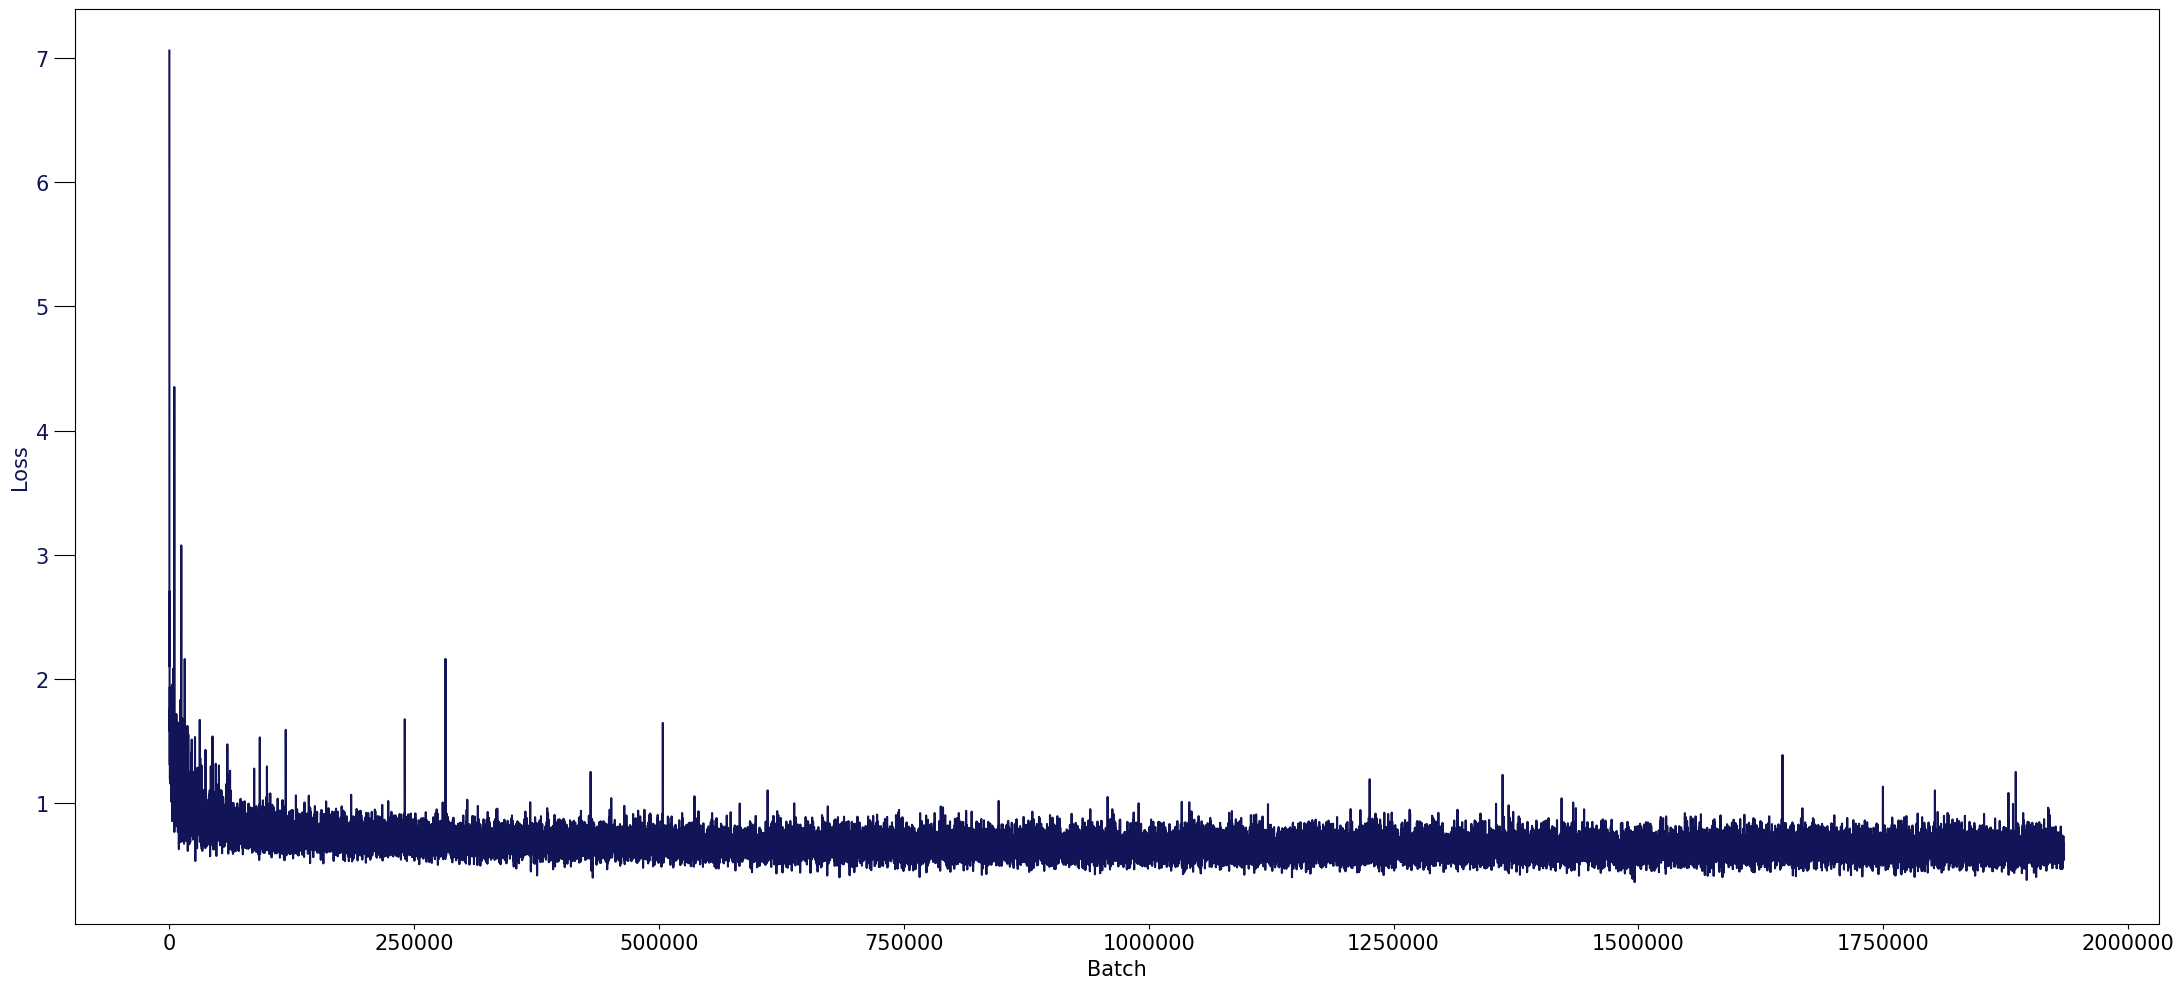
\includegraphics[width=0.9\linewidth]{Thesis//bilder/Loss-Start.png}
    \caption{Fehler-Verlauf zu Beginn}
    \label{fig:loss_start}
\end{figure}

\pagebreak
Nach den ersten Durchläufen mit den \hyperref[tab:hp_begin]{Start-Hyperparametern} ist der Fehler-Verlauf von \cref{fig:loss_start} entstanden.
Es lassen sich drei Aspekte identifizieren:
\begin{enumerate}[noitemsep]
    \item \textbf{Die Fehlerkurve rauscht}: Die Ursache ist in der Mini-Batch-Verarbeitung zu begründen. Dabei ändern sie die Daten konstant, wodurch auch der Fehler variiert. Das ist positiv und sollte auch erreicht werden, da hierdurch lokale Minima umgangen werden können \cite{Goodfellow2016}.
    \item \textbf{Der Fehler sinkt stark nach dem Beginn des Trainings}: Das liegt einerseits daran, dass das Modell mit zufälligen Gewichten initialisiert wird, daher der Fehler sehr hoch ist und auch die Anpassungen durch die Gradienten sehr hoch sind. Andererseits kann es auch an der Lernrate liegen. Diese könnte zu hoch eingestellt sein, weshalb die Anpassungen zu hoch wären.
    
    \item \textbf{Fehler stagniert nach wenigen Iterationen}: Dies kann darauf hindeuten, dass die Kapazität des Modells zu gering ist und es zu Underfitting kommt.
\end{enumerate}

Da der Fehler schnell stagniert, wurde die Epochenzahl erstmal nicht erhöht, da dadurch keine signifikante Verringerung des Fehlers erreicht wird.  
Um dem Underfitting entgegenzuwirken und die Kapazität des Netzes zu erhöhen, wurde die Modellstruktur angepasst.
Es wurde die Schichtanzahl erhöht, wobei die Struktur von $1024 \rightarrow 512 \rightarrow 256 \rightarrow 128 \rightarrow 64 \rightarrow 1$ Schichten festgelegt wurde. 

Die Lernrate, Dropout-Rate und Batch-Größe wurde nicht nur nach der Fehlerkurve optimiert. 
Die einzelnen Parameter wurden leicht variiert. 
Mit den geänderten Parametern wurde das Modell ausgeführt und danach ausgewertet.
Dieses Vorgehen diente dazu, festzulegen, wie ein Parameter geändert werden sollte

\begin{wrapfigure}[10]{r}{0.5\textwidth}
    \centering
    \captionsetup{type=table}
    \begin{tabular}{cp{4cm}}
        \hline\hline
        \thead{Hyperparameter}& Endwert\\
        \hline
        Schichtstruktur& $1024 \rightarrow 512 \rightarrow 256 \rightarrow 128 \rightarrow 64 \rightarrow 1$\\
        Dropout-Rate&$0.1$\\
        Batch-Größe&$512$\\
        Lernrate&$0.001$\\
        Epochenanzahl&$400$\\
        \hline\hline
        \end{tabular}
    \caption{Hyperparameter zu Begin}
    \label{tab:hp_end}
\end{wrapfigure}

Die Lernrate blieb unverändert, da bei einer Erhöhung das Modell nur langsamer trainiert wurde, bei einer Senkung das Rauschen zu hoch wurde.
Die Batch-Größe wurde mit der steigenden Schichtanzahl ebenfalls erhöht. 
Das hat damit zu tun, dass tiefere Netze instabilere Gradienten haben.
Um diesem Problem entgegenzuwirken, wurde mehr Stabilität durch eine höhere Batch-Größe erzeugt. 
Zusätzlich wurde die Dropout-Rate auf $0.1$ abgesenkt, da hierdurch die Bewertung besser geworden ist.

Mit diesen Änderungen wurde dann folgende Fehlerkurve erreicht:
\begin{figure}[H]
    \centering
    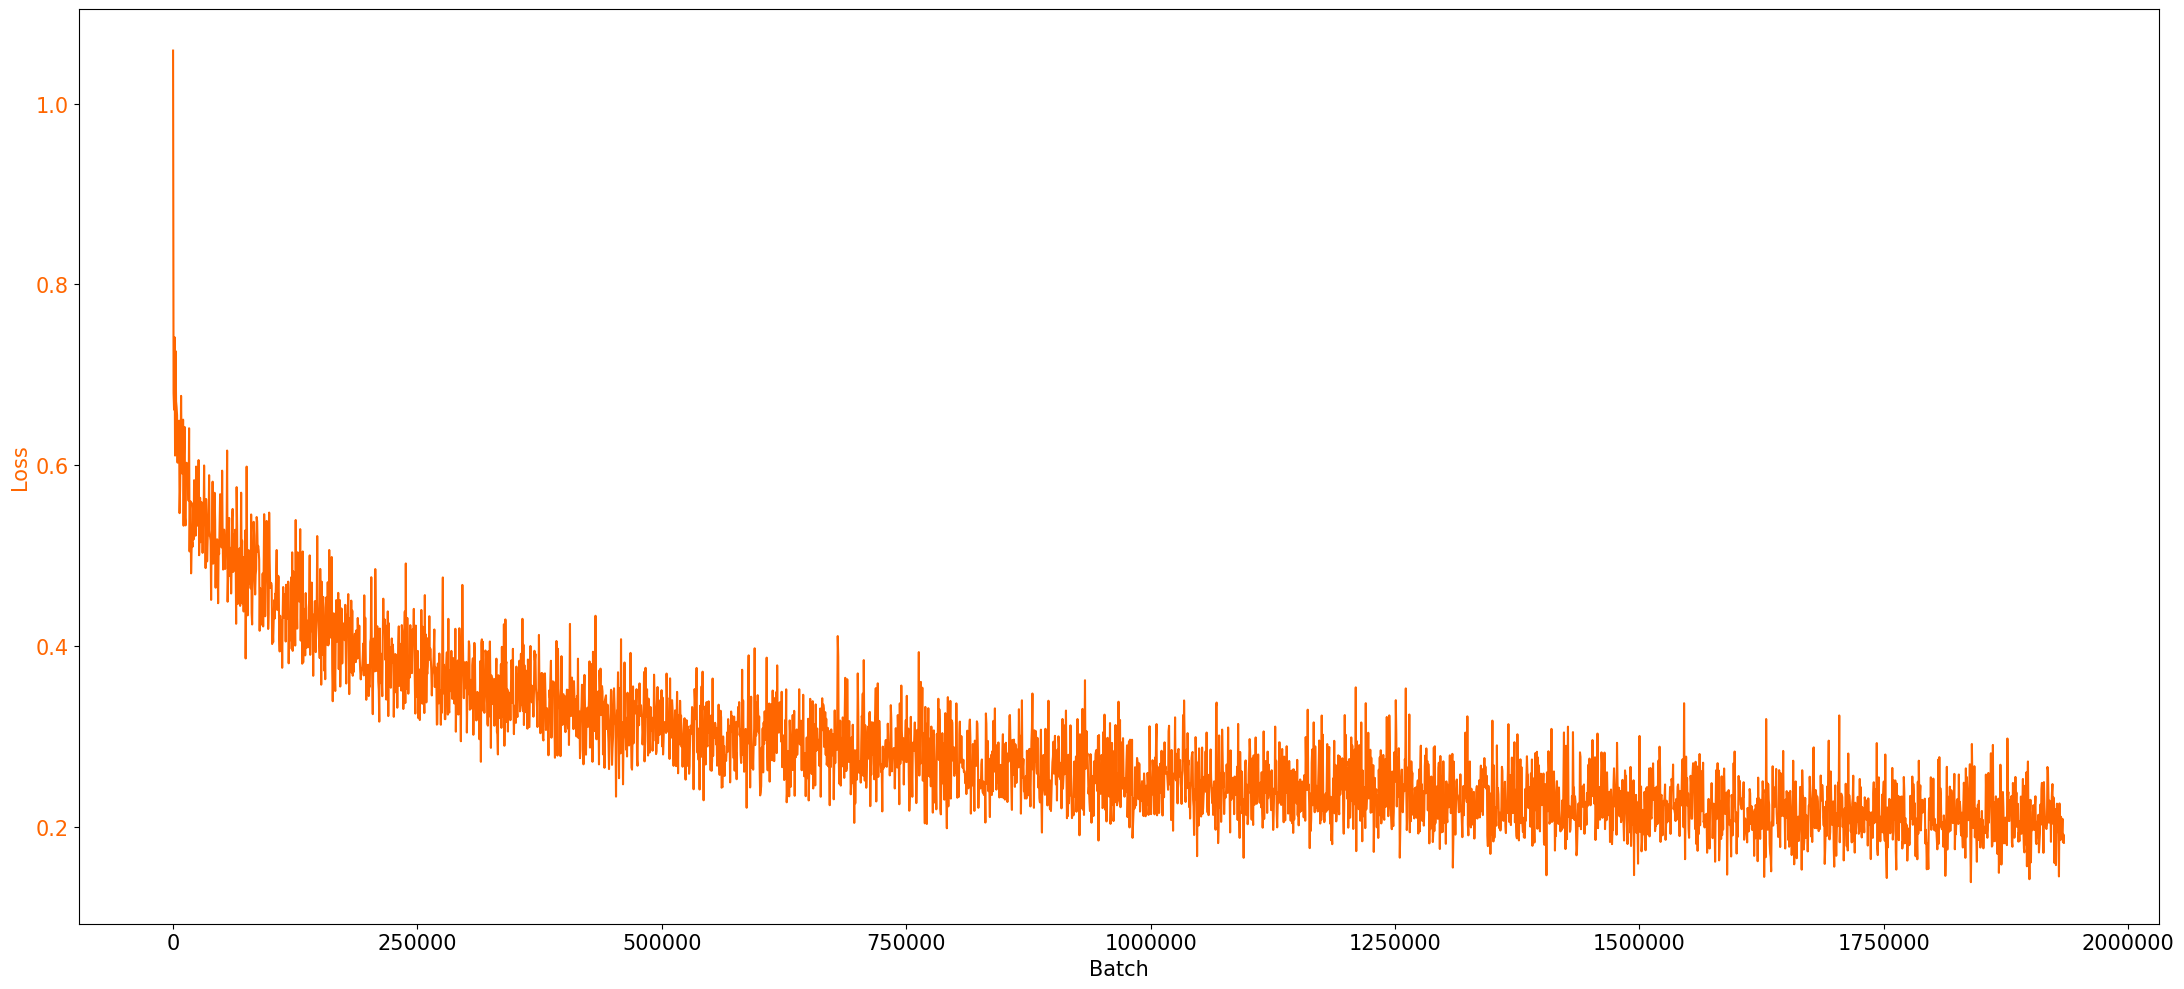
\includegraphics[width=0.9\linewidth]{Thesis//bilder/Loss-End.png}
    \caption{Fehler-Verlauf zu Ende}
    \label{fig:loss_end}
\end{figure}

Mit den finalen Parametern benötigt das Modell eine Trainingszeit von ca. $12$ Stunden.

Die Auswertung, wie das Modell nach dem Training ausgewertet wurde, wird in \cref{ref:auswertung} erläutert.

\subsection{Random Forest}
\label{sec:impl_rf}

%sklean
%Erklären das es zum vergleichen genutzt wurde
%Bezug zu Theoriekapitel
%Einfachere Methode
%Wie schon erwähnt gleicher Aufbau
%Conatinertypen und Special Products wurden auch per Feature Engeneering umgewandelt, da es verständlicher in der Darstellung ist

%\todo{IW: Warum nur Teiweise?}
%Später stellt sich heraus, dass Random Forest hier viel besser ist als neuronale Netze. Warum also nur "teilweise"?

%\todo{IW: Wie hoch ist die Ausführungszeit?}
%Wie hoch ist das denn? Sind die Ausführungszeiten relevant?
%Wenn das im Millisekundenbereich ist, dass würde ja sogar der Faktor 100 keine Rolle spielen.

%Warum Random Forest
% -> Einfacher (weniger tuning)
% -> Performanter
% -> etc.

Um die einfache Implementierung auszunutzen, wurde das \enquote{scikit-learn} Framework verwendet.

Die Anfangsstruktur für das Random Forest-Training ist gleich wie auch in den neuronalen Netzen:
Es werden die Daten aus der \enquote{waitinglist\_data} Tabelle per \enquote{PySpark} in einen Dataframe geladen.
Daraufhin wird direkt das \hyperref[sec:feature_engeneering]{Feature Engeneering} ausgeführt.

Die Implementierung des Random Forest-Algorithmus in \enquote{scikit-learn} kann ausschließlich numerische Werte verarbeiten.  
Daher war es erforderlich, die kategorialen Textdaten in numerische Werte zu kodieren.

Für den Random Forest wurde, wie beim neuronalen Netz, die One-Hot-Kodierung verwendet.  
Für Kategorien mit einer höheren Kardinalität (siehe \ref{tab:enc_features}) wurde jedoch Zielkodierung implementiert.
Die Kodierungen kann auch mit dem \enquote{scikit-learn}-Framework durchgeführt werden. 
Dafür werden die Daten wieder in Trainings- und Testdaten eingeteilt und anschließend die Zeilen mittels \href{https://scikit-learn.org/stable/modules/generated/sklearn.preprocessing.OneHotEncoder.html}{\enquote{OneHotEncoder}} und \href{https://scikit-learn.org/stable/modules/generated/sklearn.preprocessing.TargetEncoder.html}{\enquote{TargetEncoder}} kodiert.

Im Anschluss daran sind die Daten fertig vorverarbeitet für das Training, da für den Random Forest-Algorithmus keine weiteren Parameter bestimmt werden müssen. 

Das \enquote{scikit-learn}-Framework vereinfacht das Training, indem lediglich eine Instanz vom \href{https://scikit-learn.org/stable/modules/generated/sklearn.ensemble.RandomForestClassifier.html}{\enquote{RandomForestClassifier}} initialisiert wird. An diesen müssen für das Training nur noch die Trainingsdaten sowie die Zieldaten übergeben werden.
Nach der Trainingszeit kann der trainierte \href{https://scikit-learn.org/stable/modules/generated/sklearn.ensemble.RandomForestClassifier.html}{\enquote{RandomForestClassifier}} Vorhersagen für die Testdaten machen.

Dabei kann gewählt werden, ob reine Vorhersagen oder ob eine Wahrscheinlichkeit ausgeben werden soll. 
Für das binäre Klassifizierungsproblem wurde die Wahrscheinlichkeit gewählt.

Das Training dauert nur etwa $45$ Minuten. Im Vergleich zum neuronalen Netz entspricht das lediglich $6\text{,}25\%$ der Trainingszeit und bedeutet somit eine Zeitersparnis von fast $94\%$.
%\todo{IW: Ausführungszeit?!}
%Das bedeutet, dass Sie für neuronale Netze mehr als 10 Stunden trainieren müssen?
%Das finde ich schon erheblich!

\subsection{Logistische Regression}
\label{sec:impl_log_reg}

Das \enquote{scikit-learn}-Framework kann auch für die logistische Regression verwendet werden, weshalb es aufgrund der einfachen Implementierung gewählt wurde. 
Als Grundkonstrukt wurde das Random Forest-Notebook verwendet, die Struktur ist also grundlegend gleich.
\begin{enumerate}[noitemsep]
    \item Laden der Daten aus der \enquote{waitinglist\_data} Tabelle per \enquote{PySpark} in einen Dataframe
    \item Ausführung des \hyperref[sec:feature_engeneering]{Feature Engeneering}
    \item Training der logistischen Regression
\end{enumerate}

Wie beim Random Forest können auch bei der logistischen Regression mit \enquote{scikit-learn} ausschließlich numerische Werte verarbeitet werden.
Daher war es erforderlich, die kategorischen Textdaten in numerische Werte zu kodieren.
Die Kodierung wurde vollständig vom Random Forest übernommen, es wurde also die One-Hot-Kodierung und für höhere Kardinalität (siehe \ref{tab:enc_features}) Zielwertkodierung implementiert.

Für das Training wurde lediglich eine 
\href{https://scikit-learn.org/stable/modules/generated/sklearn.linear_model.LogisticRegression.html}{LogisticRegression}
Instanz erzeugt. Hierbei kann dann das Optimierungsverfahren mit dem \enquote{solver}-Parameter eingestellt werden.
Es wurde das Newton-CG-Verfahren gewählt, da es eine effiziente Balance zwischen Konvergenzgeschwindigkeit und Rechenaufwand bietet. Während klassische Newton-Verfahren eine explizite Berechnung und Inversion der Hesse-Matrix erfordern, vermeidet Newton-CG diesen hohen Speicher- und Rechenaufwand, indem es die Hesse-Matrix nur implizit in Kombination mit konjugierten Gradienten verwendet \cite{Minka2003}. 
Laut Minka \cite{Minka2003} gehört Newton-CG zu den leistungsfähigsten Verfahren für hochdimensionale Daten, da es eine zweite Ordnungsmethode mit verbesserter numerischer Stabilität ist, aber gleichzeitig auf speicherintensive Matrixinversionen verzichtet. 

Nach der Initialisierung wurden die kodierten Daten an die
\href{https://scikit-learn.org/stable/modules/generated/sklearn.linear_model.LogisticRegression.html#sklearn.linear_model.LogisticRegression.fit}{\enquote{fit}}-Funktion übergeben und das Training hiermit gestartet.

Wie üblich für das \enquote{scikit-learn}-Framework, kann nach dem Training mit der 
\href{https://scikit-learn.org/stable/modules/generated/sklearn.linear_model.LogisticRegression.html#sklearn.linear_model.LogisticRegression.predict_proba}{\enquote{predict\_proba}}-Methode die Wahrscheinlichkeiten vorhergesagt werden.

Das Training dauerte in diesem Fall $37$ Minuten und war damit kürzer als die $45$ Minuten beim Random Forest. 
Im Vergleich zum neuronalen Netz entspricht das noch $5\text{,}14\%$ der Zeit, was einer Zeitersparnis von fast $95\%$ entspricht.

\subsection{Compute-Cluster}
Das neuronale Netz, das Random Forest-Modell sowie die logistische Regression wurden in \nameref{sec:databricks}-Python-Notebooks ausgeführt. 
Jedes Notebook wird dabei mit einem Compute-Cluster verbunden, auf dem die entsprechenden Notebooks ausgeführt werden. 
Zur Beurteilung, ob die Ausführungszeit durch die verwendete Hardware beeinflusst wurde, wird in diesem Abschnitt die eingesetzte Hardware spezifiziert.

\pagebreak
Für das Cluster wurde eine \gls{aws} EC2 \enquote{m5d.8xlarge}-Instanz verwendet. Diese bietet die folgenden Spezifikationen:

\begin{table}[H]
    \centering
    \begin{tabular}{lr}
        \hline\hline
        \thead{\textbf{Eigenschaft}}&\textbf{Wert}\\
        \hline
        \glspl{vcpu}& 32 \\
        Arbeitspeicher (GiB)& 128.0 \\
        Arbeitspeicher pro vCPU (GiB)& 4.0 \\
        Physischer Prozessor& Intel Xeon Platinum 8175 \\
        Tacktrate (GHz)& 3.1 \\
        \gls{cpu} Architecture& x86\_64 \\
        \gls{gpu} Anzahl& 0 \\
        \hline\hline
    \end{tabular}
    \caption{Compute-Cluster: Hardware-Eigenschaften}
    \label{tab:cc_hardware_props}
\end{table}

Es wurde kein \gls{gpu} Training verwendet. Dies wurde beim Training des neuronalen Netzes überprüft und zeigte keinen wesentlichen Einfluss auf die Performance.

Diese Hardware kostet $2\text{,}176\ \$$ pro Stunde \cite{awspricing}. Bei einem neuronalen Netz, mit einer Ausführungszeit von $12$ Stunden, kostet also ein Training alleine $26\text{,}112\ \$$. Beim Random Forest-Modell kostet ein Training nur $1\text{,}632\ \$$, da es nur $45$ Minuten trainiert. 
Die logistische Regression ist aufgrund der kurzen Trainingszeit von $37$ Minuten mit $1\text{,}34\ \$$ das kostengünstigste Modell.